\begin{bw_box}
\begin{customproblem}{Π1}
  \label{prob:02_02:the_problem}
  Έστω ένα ρομπότ κινητής βάσης ικανό να κινείται στο επίπεδο $x-y$ εξοπλισμένο
  με έναν οριζόντια τοποθετημένο αισθητήρα lidar μετρήσεων δύο διαστάσεων
  που εκπέμπει $N_s$ ακτίνες. Έστω επίσης τα ακόλουθα να είναι διαθέσιμα ή να
  ευσταθούν:
  \begin{itemize}
    \item Ο χάρτης $\bm{M}$ του περιβάλλοντος στο οποίο κινείται το ρομπότ
    \item Μια δισδιάστατη μέτρηση $\mathcal{S}_R$, που λαμβάνεται από
          την---άγνωστη και αναζητούμενη---στάση $\bm{p}(\bm{l},\theta)$,
          $\bm{l} = (x,y)$
    \item Μια εκτίμηση της θέσης του αισθητήρα
          $\hat{\bm{p}}(\hat{\bm{l}}, \hat{\theta})$ στο σύστημα αναφοράς του
          χάρτη, όπου $\hat{\bm{l}} = (\hat{x}, \hat{y})$ είναι σε μία γειτονιά
          του $\bm{l}$
  \end{itemize}
\end{customproblem}
Τότε ο στόχος είναι να μειωθεί το μέγεθος του σφάλματος στάσης του αισθητήρα
$\bm{e}(\bm{p}, \hat{\bm{p}}) \triangleq \bm{p}- \hat{\bm{p}}$ από την αρχική
του τιμή
\begin{align}
  \|\bm{e}(\bm{p}, \hat{\bm{p}})\|_2 = ((x- \hat{x})^2 + (y- \hat{y})^2 + (\theta- \hat{\theta})^2)^{1/2}
  \label{eq:pose_error_def}
\end{align}
βελτιώνοντας την εκτίμηση της στάσης του αισθητήρα σε
$\hat{\bm{p}}^\prime(\hat{x}^\prime, \hat{y}^\prime, \hat{\theta}^\prime)$ έτσι ώστε
\begin{align}
  \|\bm{e}(\bm{p}, \hat{\bm{p}}^\prime)\|_2 < \|\bm{e}(\bm{p}, \hat{\bm{p}})\|_2
  \tag{$\ast$}
  \label{obj:the_objective}
\end{align}
\end{bw_box}
Υποθέτοντας ότι η στάση του αισθητήρα σε σχέση με το σύστημα αναφοράς του
ρομπότ είναι γνωστή, η διόρθωση της εκτίμησης της στάσης του αισθητήρα είναι
ίση με το διόρθωση της εκτίμησης της στάσης του ρομπότ σε σχέση με το σύστημα
αναφοράς του χάρτη. Ένα παράδειγμα μιας συνήθους συνθήκης του προβλήματος
\ref{prob:02_02:the_problem} απεικονίζεται στο σχήμα
\ref{fig:02_02:the_problem}. Η εκτίμηση της στάσης $\hat{\bm{p}}$
παρέχεται εξωτερικά από ένα σύστημα εντοπισμού στην περίπτωση της
παρακολούθησης της στάσης, ή ως υπόθεση στάσης στην περίπτωση του προβλήματος
εύρεσης της στάσης του ρομπότ βάσει καθολικής αβεβαιότητος.

\begin{figure}[]\centering
  % GNUPLOT: LaTeX picture with Postscript
\begingroup
  \makeatletter
  \providecommand\color[2][]{%
    \GenericError{(gnuplot) \space\space\space\@spaces}{%
      Package color not loaded in conjunction with
      terminal option `colourtext'%
    }{See the gnuplot documentation for explanation.%
    }{Either use 'blacktext' in gnuplot or load the package
      color.sty in LaTeX.}%
    \renewcommand\color[2][]{}%
  }%
  \providecommand\includegraphics[2][]{%
    \GenericError{(gnuplot) \space\space\space\@spaces}{%
      Package graphicx or graphics not loaded%
    }{See the gnuplot documentation for explanation.%
    }{The gnuplot epslatex terminal needs graphicx.sty or graphics.sty.}%
    \renewcommand\includegraphics[2][]{}%
  }%
  \providecommand\rotatebox[2]{#2}%
  \@ifundefined{ifGPcolor}{%
    \newif\ifGPcolor
    \GPcolorfalse
  }{}%
  \@ifundefined{ifGPblacktext}{%
    \newif\ifGPblacktext
    \GPblacktexttrue
  }{}%
  % define a \g@addto@macro without @ in the name:
  \let\gplgaddtomacro\g@addto@macro
  % define empty templates for all commands taking text:
  \gdef\gplbacktext{}%
  \gdef\gplfronttext{}%
  \makeatother
  \ifGPblacktext
    % no textcolor at all
    \def\colorrgb#1{}%
    \def\colorgray#1{}%
  \else
    % gray or color?
    \ifGPcolor
      \def\colorrgb#1{\color[rgb]{#1}}%
      \def\colorgray#1{\color[gray]{#1}}%
      \expandafter\def\csname LTw\endcsname{\color{white}}%
      \expandafter\def\csname LTb\endcsname{\color{black}}%
      \expandafter\def\csname LTa\endcsname{\color{black}}%
      \expandafter\def\csname LT0\endcsname{\color[rgb]{1,0,0}}%
      \expandafter\def\csname LT1\endcsname{\color[rgb]{0,1,0}}%
      \expandafter\def\csname LT2\endcsname{\color[rgb]{0,0,1}}%
      \expandafter\def\csname LT3\endcsname{\color[rgb]{1,0,1}}%
      \expandafter\def\csname LT4\endcsname{\color[rgb]{0,1,1}}%
      \expandafter\def\csname LT5\endcsname{\color[rgb]{1,1,0}}%
      \expandafter\def\csname LT6\endcsname{\color[rgb]{0,0,0}}%
      \expandafter\def\csname LT7\endcsname{\color[rgb]{1,0.3,0}}%
      \expandafter\def\csname LT8\endcsname{\color[rgb]{0.5,0.5,0.5}}%
    \else
      % gray
      \def\colorrgb#1{\color{black}}%
      \def\colorgray#1{\color[gray]{#1}}%
      \expandafter\def\csname LTw\endcsname{\color{white}}%
      \expandafter\def\csname LTb\endcsname{\color{black}}%
      \expandafter\def\csname LTa\endcsname{\color{black}}%
      \expandafter\def\csname LT0\endcsname{\color{black}}%
      \expandafter\def\csname LT1\endcsname{\color{black}}%
      \expandafter\def\csname LT2\endcsname{\color{black}}%
      \expandafter\def\csname LT3\endcsname{\color{black}}%
      \expandafter\def\csname LT4\endcsname{\color{black}}%
      \expandafter\def\csname LT5\endcsname{\color{black}}%
      \expandafter\def\csname LT6\endcsname{\color{black}}%
      \expandafter\def\csname LT7\endcsname{\color{black}}%
      \expandafter\def\csname LT8\endcsname{\color{black}}%
    \fi
  \fi
    \setlength{\unitlength}{0.0500bp}%
    \ifx\gptboxheight\undefined%
      \newlength{\gptboxheight}%
      \newlength{\gptboxwidth}%
      \newsavebox{\gptboxtext}%
    \fi%
    \setlength{\fboxrule}{0.5pt}%
    \setlength{\fboxsep}{1pt}%
\begin{picture}(4000.00,4000.00)%
    \gplgaddtomacro\gplbacktext{%
      \colorrgb{0.15,0.15,0.15}%
      \put(462,583){\makebox(0,0)[r]{\strut{}$7.0$}}%
      \colorrgb{0.15,0.15,0.15}%
      \put(462,1013){\makebox(0,0)[r]{\strut{}$8.0$}}%
      \colorrgb{0.15,0.15,0.15}%
      \put(462,1443){\makebox(0,0)[r]{\strut{}$9.0$}}%
      \colorrgb{0.15,0.15,0.15}%
      \put(462,1873){\makebox(0,0)[r]{\strut{}$10.0$}}%
      \colorrgb{0.15,0.15,0.15}%
      \put(462,2302){\makebox(0,0)[r]{\strut{}$11.0$}}%
      \colorrgb{0.15,0.15,0.15}%
      \put(462,2732){\makebox(0,0)[r]{\strut{}$12.0$}}%
      \colorrgb{0.15,0.15,0.15}%
      \put(462,3162){\makebox(0,0)[r]{\strut{}$13.0$}}%
      \colorrgb{0.15,0.15,0.15}%
      \put(462,3592){\makebox(0,0)[r]{\strut{}$14.0$}}%
      \colorrgb{0.15,0.15,0.15}%
      \put(594,363){\makebox(0,0){\strut{}$2.0$}}%
      \colorrgb{0.15,0.15,0.15}%
      \put(1024,363){\makebox(0,0){\strut{}$3.0$}}%
      \colorrgb{0.15,0.15,0.15}%
      \put(1454,363){\makebox(0,0){\strut{}$4.0$}}%
      \colorrgb{0.15,0.15,0.15}%
      \put(1884,363){\makebox(0,0){\strut{}$5.0$}}%
      \colorrgb{0.15,0.15,0.15}%
      \put(2313,363){\makebox(0,0){\strut{}$6.0$}}%
      \colorrgb{0.15,0.15,0.15}%
      \put(2743,363){\makebox(0,0){\strut{}$7.0$}}%
      \colorrgb{0.15,0.15,0.15}%
      \put(3173,363){\makebox(0,0){\strut{}$8.0$}}%
      \colorrgb{0.15,0.15,0.15}%
      \put(3603,363){\makebox(0,0){\strut{}$9.0$}}%
      \put(2000,63){\makebox(0,0){\strut{}$x$ [m]}}%
      \put(-163,2000){\rotatebox{90}{\makebox(0,0)[r]{\strut{}$y$ [m]}}}%
    }%
    \gplgaddtomacro\gplfronttext{%
      \colorrgb{0.00,0.00,0.00}%
      \put(2954,884){\makebox(0,0)[l]{\strut{}$\bm{p}$}}%
      \put(2657,884){\makebox(0,0)[l]{\strut{}$\hat{\bm{p}}$}}%
    }%
    \gplbacktext
    \put(0,0){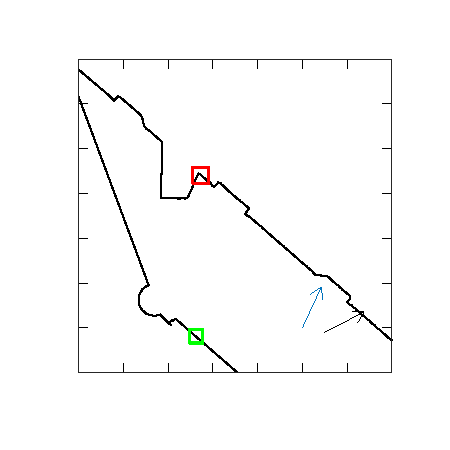
\includegraphics{./figures/parts/02/chapters/02/sections/01/problem}}%
    \gplfronttext
  \end{picture}%
\endgroup

  \caption{\small Μια επί της αρχής τυπική συνθήκη εντοπισμού: Η πραγματική
           στάση του ρομπότ είναι $\bm{p}$ αλλά η εκτίμησή της
           $\hat{\bm{p}}^\prime$ είναι μετατοπισμένη ως προς τη θέση και τον
           προσανατολισμό. Ο ρυθμός των μεταβολών του τμήματος του
           περιβάλλοντος που περιβάλλεται με κόκκινο χρώμα είναι μεγαλύτερος
           από από εκείνον του τμήματος που περιβάλλεται με πράσινο}
  \label{fig:02_02:the_problem}
\end{figure}
